% questions.tex —— 2007 年·春季上海卷 · 题目内容片段（无答案）
% 由 tools/generate_projects.py 依来源总账自 2007/2007_数学真题_春季上海_试题.md 生成，勿手改（改源 MD 后重跑）


\begin{gktip}
\textbf{来源说明}：题面按固定PDF第1–3页转录，另由未撰写首稿的复核者逐题对照原页；图形重绘为TikZ，表格使用原生LaTeX。第4–6页印载参考答案另行归档，不认证官方身份。本库答案为仅依据题面盲解后复核整理的独立推导，官方答案字段保持空值。

\textbf{页码映射}：Q1–5在PDF1，Q6跨PDF1–2，Q7–16在PDF2，Q17跨PDF2–3，Q18–21在PDF3。题数21、满分150、考试时间120分钟；分值及小问分值按源卷保留。
\end{gktip}

\gkpart{考生注意}

1. 答卷前，考生务必将姓名、高考座位号、校验码等填写清楚。
2. 本试卷共有21道试题，满分150分。考试时间120分钟。

\gkpart{一、填空题（本大题满分44分）}

本大题共有11题，只要求直接填写结果，每题填对得4分，否则一律得零分。

\begin{question}
\gkti{1}\textbf{（本题满分 $4$ 分）} 计算 $\displaystyle\lim_{n\to\infty}\frac{2n^2+1}{3n(n+1)}=$ $\underline{\qquad\qquad}$。

\end{question}
\begin{question}
\gkti{2}\textbf{（本题满分 $4$ 分）} 若关于 $x$ 的一元二次实系数方程 $x^2+px+q=0$ 有一个根为 $1+\mathrm{i}$（$\mathrm{i}$ 是虚数单位），则 $q=$ $\underline{\qquad\qquad}$。

\end{question}
\begin{question}
\gkti{3}\textbf{（本题满分 $4$ 分）} 若关于 $x$ 的不等式 $\dfrac{x-a}{x+1}>0$ 的解集为 $(-\infty,-1)\cup(4,+\infty)$，则实数 $a=$ $\underline{\qquad\qquad}$。

\end{question}
\begin{question}
\gkti{4}\textbf{（本题满分 $4$ 分）} 函数 $y=(\sin x+\cos x)^2$ 的最小正周期为 $\underline{\qquad\qquad}$。

\end{question}
\begin{question}
\gkti{5}\textbf{（本题满分 $4$ 分）} 设函数 $y=f(x)$ 是奇函数。若 $f(-2)+f(-1)-3=f(1)+f(2)+3$，则 $f(1)+f(2)=$ $\underline{\qquad\qquad}$。

\end{question}
\begin{question}
\gkti{6}\textbf{（本题满分 $4$ 分）} 在平面直角坐标系 $xOy$ 中，若抛物线 $y^2=4x$ 上的点 $P$ 到该抛物线的焦点的距离为6，则点 $P$ 的横坐标 $x=$ $\underline{\qquad\qquad}$。

\end{question}
\begin{question}
\gkti{7}\textbf{（本题满分 $4$ 分）} 在平面直角坐标系 $xOy$ 中，若曲线 $x=\sqrt{4-y^2}$ 与直线 $x=m$ 有且只有一个公共点，则实数 $m=$ $\underline{\qquad\qquad}$。

\end{question}
\begin{question}
\gkti{8}\textbf{（本题满分 $4$ 分）} 若向量 $\vec a$、$\vec b$ 满足 $|\vec a|=\sqrt2$，$|\vec b|=1$，$\vec a\cdot(\vec a+\vec b)=1$，则向量 $\vec a$、$\vec b$ 的夹角的大小为 $\underline{\qquad\qquad}$。

\end{question}
\begin{question}
\gkti{9}\textbf{（本题满分 $4$ 分）} 若 $x_1$、$x_2$ 为方程 $2^x=\left(\dfrac12\right)^{-\frac1x+1}$ 的两个实数解，则 $x_1+x_2=$ $\underline{\qquad\qquad}$。

\end{question}
\begin{question}
\gkti{10}\textbf{（本题满分 $4$ 分）} 在一次教师联欢会上，到会的女教师比男教师多12人，从这些教师中随机挑选一人表演节目。若选到男教师的概率为 $\dfrac9{20}$，则参加联欢会的教师共有 $\underline{\qquad\qquad}$ 人。

\end{question}
\begin{question}
\gkti{11}\textbf{（本题满分 $4$ 分）} 函数 $y=\begin{cases}x^2+1,&x\geq0,\\ \dfrac2x,&x<0\end{cases}$ 的反函数是 $\underline{\qquad\qquad}$。

\end{question}
\gkpart{二、选择题（本大题满分16分）}

本大题共有4题，每题都给出四个结论，其中有且只有一个结论是正确的，必须把正确结论的代号写在题后的圆括号内，选对得4分，否则一律得零分。

\begin{question}
\gkti{12}\textbf{（本题满分 $4$ 分）} 若集合 $A=\{1,m^2\}$，$B=\{2,4\}$，则“$m=2$”是“$A\cap B=\{4\}$”的

（A） 充分不必要条件。

（B） 必要不充分条件。

（C） 充要条件。

（D） 既不充分也不必要条件。

[答]（　）

\Needspace{0.4\textheight}
\end{question}
\begin{question}
\gkti{13}\textbf{（本题满分 $4$ 分）} 如图，平面内的两条相交直线 $OP_1$ 和 $OP_2$ 将该平面分割成四个部分 I、II、III、IV（不包括边界）。若 $\overrightarrow{OP}=a\overrightarrow{OP_1}+b\overrightarrow{OP_2}$，且点 $P$ 落在第III部分，则实数 $a$、$b$ 满足
\nopagebreak[4]
\begin{center}% Q13: source PDF p2; intersecting lines have no arrows.
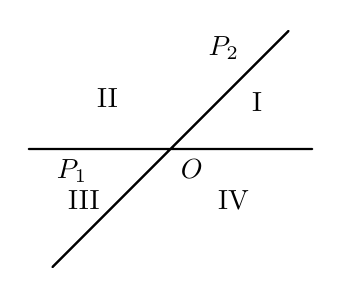
\begin{tikzpicture}[line cap=round,line join=round,thick]
\draw (-1.8,0)--(1.8,0) (-1.5,-1.5)--(1.5,1.5);
\node[below right] at (0,0) {$O$};
\node[below] at (-1.25,0) {$P_1$};
\node[above left] at (1,1) {$P_2$};
\node at (1.1,.6) {I}; \node at (-.8,.65) {II};
\node at (-1.1,-.65) {III}; \node at (.8,-.65) {IV};
\end{tikzpicture}
\end{center}
\nopagebreak[4]
（A） $a>0,b>0$。

（B） $a>0,b<0$。

（C） $a<0,b>0$。

（D） $a<0,b<0$。

[答]（　）

\Needspace{0.4\textheight}
\end{question}
\begin{question}
\gkti{14}\textbf{（本题满分 $4$ 分）} 下列四个函数中，图象如图所示的只能是

（A） $y=x+\lg x$。

（B） $y=x-\lg x$。

（C） $y=-x+\lg x$。

（D） $y=-x-\lg x$。
\nopagebreak[4]
\begin{center}% Q14: source PDF p2; unticked qualitative curve, no equation label.
\begin{tikzpicture}[line cap=round,line join=round,thick]
\draw[->] (-.45,0)--(3.15,0) node[right] {$x$};
\draw[->] (0,-.45)--(0,2.65) node[above] {$y$};
\draw[domain=-3:.45,samples=150,smooth] plot ({10^(\x)},{.65*(10^(\x)-\x)});
\node[below left] at (0,0) {$O$};
\end{tikzpicture}
\end{center}
\nopagebreak[4]
[答]（　）

\end{question}
\begin{question}
\gkti{15}\textbf{（本题满分 $4$ 分）} 设 $a$、$b$ 是正实数，以下不等式

① $\sqrt{ab}>\dfrac{2ab}{a+b}$，② $a>|a-b|-b$，③ $a^2+b^2>4ab-3b^2$，④ $ab+\dfrac2{ab}>2$ 恒成立的序号为

（A） ①、③。

（B） ①、④。

（C） ②、③。

（D） ②、④。

[答]（　）

\end{question}
\gkpart{三、解答题（本大题满分90分）}

本大题共有6题，解答下列各题必须写出必要的步骤。

\Needspace{0.4\textheight}
\begin{question}
\gkti{16}\textbf{（本题满分 $12$ 分）} 如图，在棱长为2的正方体 $ABCD-A'B'C'D'$ 中，$E$、$F$ 分别是 $A'B'$ 和 $AB$ 的中点，求异面直线 $A'F$ 与 $CE$ 所成角的大小（结果用反三角函数值表示）。
\nopagebreak[4]
\begin{center}% Q16: source PDF p2; hidden AD, DC, DD' and EC dashed.
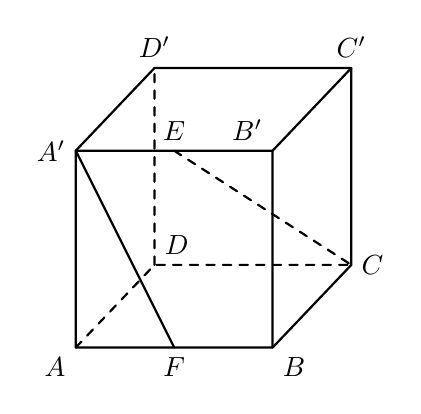
\begin{tikzpicture}[line cap=round,line join=round,thick]
\coordinate (A) at (0,0); \coordinate (B) at (2.5,0);
\coordinate (C) at (3.5,1.05); \coordinate (D) at (1,1.05);
\coordinate (Ap) at (0,2.5); \coordinate (Bp) at (2.5,2.5);
\coordinate (Cp) at (3.5,3.55); \coordinate (Dp) at (1,3.55);
\coordinate (E) at (1.25,2.5); \coordinate (F) at (1.25,0);
\draw[dashed] (A)--(D)--(C) (D)--(Dp) (E)--(C);
\draw (A)--(B)--(C)--(Cp)--(Dp)--(Ap)--cycle;
\draw (Ap)--(Bp)--(Cp) (B)--(Bp) (Ap)--(F);
\node[below left] at (A) {$A$}; \node[below right] at (B) {$B$};
\node[right] at (C) {$C$}; \node[above right] at (D) {$D$};
\node[left] at (Ap) {$A'$}; \node[above left] at (Bp) {$B'$};
\node[above] at (Cp) {$C'$}; \node[above] at (Dp) {$D'$};
\node[above] at (E) {$E$}; \node[below] at (F) {$F$};
\end{tikzpicture}
\end{center}
\nopagebreak[4]
\end{question}
\begin{question}
\gkti{17}\textbf{（本题满分 $14$ 分）} 求出一个数学问题的正确结论后，将其作为条件之一，提出与原来问题有关的新问题，我们把它称为原来问题的一个“逆向”问题。

例如，原来问题是“若正四棱锥底面边长为4，侧棱长为3，求该正四棱锥的体积”。求出体积 $\dfrac{16}3$ 后，它的一个“逆向”问题可以是“若正四棱锥底面边长为4，体积为 $\dfrac{16}3$，求侧棱长”；也可以是“若正四棱锥的体积为 $\dfrac{16}3$，求所有侧面面积之和的最小值”。

试给出问题“在平面直角坐标系 $xOy$ 中，求点 $P(2,1)$ 到直线 $3x+4y=0$ 的距离”的一个有意义的“逆向”问题，并解答你所给出的“逆向”问题。

\Needspace{0.4\textheight}
\end{question}
\begin{question}
\gkti{18}\textbf{（本题满分 $14$ 分）} 本题共有2个小题，第1小题满分6分，第2小题满分8分。

如图，在直角坐标系 $xOy$ 中，设椭圆 $C:\dfrac{x^2}{a^2}+\dfrac{y^2}{b^2}=1$（$a>b>0$）的左右两个焦点分别为 $F_1$、$F_2$。过右焦点 $F_2$ 且与 $x$ 轴垂直的直线 $l$ 与椭圆 $C$ 相交，其中一个交点为 $M(\sqrt2,1)$。

(1) 求椭圆 $C$ 的方程；

(2) 设椭圆 $C$ 的一个顶点为 $B(0,-b)$，直线 $BF_2$ 交椭圆 $C$ 于另一点 $N$，求 $\triangle F_1BN$ 的面积。
\nopagebreak[4]
\begin{center}% Q18: source PDF p3; only the source's F1,F2,O,M,l labels.
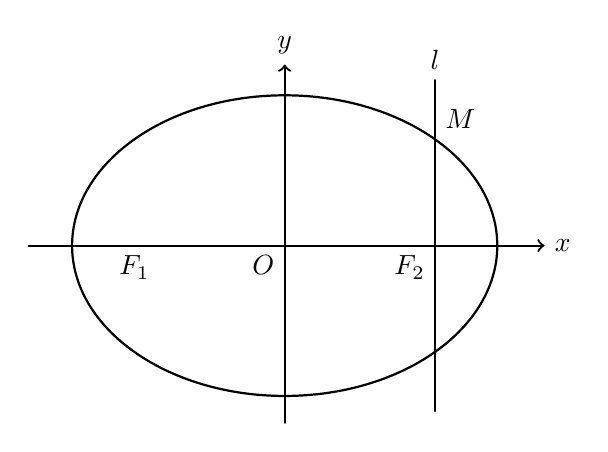
\begin{tikzpicture}[line cap=round,line join=round,thick]
\draw[->] (-3.25,0)--(3.3,0) node[right] {$x$};
\draw[->] (0,-2.25)--(0,2.3) node[above] {$y$};
\draw (0,0) ellipse (2.7 and 1.9092);
\draw (1.9092,-2.1)--(1.9092,2.1) node[above] {$l$};
\node[below left] at (0,0) {$O$};
\node[below] at (-1.9092,0) {$F_1$};
\node[below left] at (1.9092,0) {$F_2$};
\node[above right] at (1.9092,1.35) {$M$};
\end{tikzpicture}
\end{center}
\nopagebreak[4]
\Needspace{0.4\textheight}
\end{question}
\begin{question}
\gkti{19}\textbf{（本题满分 $14$ 分）} 本题共有2个小题，第1小题满分4分，第2小题满分10分。

某人定制了一批地砖。每块地砖（如图1所示）是边长为0.4米的正方形 $ABCD$，点 $E$、$F$ 分别在边 $BC$ 和 $CD$ 上，$\triangle CFE$、$\triangle ABE$ 和四边形 $AEFD$ 均由单一材料制成，制成 $\triangle CFE$、$\triangle ABE$ 和四边形 $AEFD$ 的三种材料的每平方米价格之比依次为 $3:2:1$。若将此种地砖按图2所示的形式铺设，能使中间的深色阴影部分成四边形 $EFGH$。

(1) 求证：四边形 $EFGH$ 是正方形；

(2) $E$、$F$ 在什么位置时，定制这批地砖所需的材料费用最省？
\nopagebreak[4]
\begin{center}% Q19: source PDF p3; one tile and its four rotated copies.
% Coordinates are schematic and introduce no numerical labels.
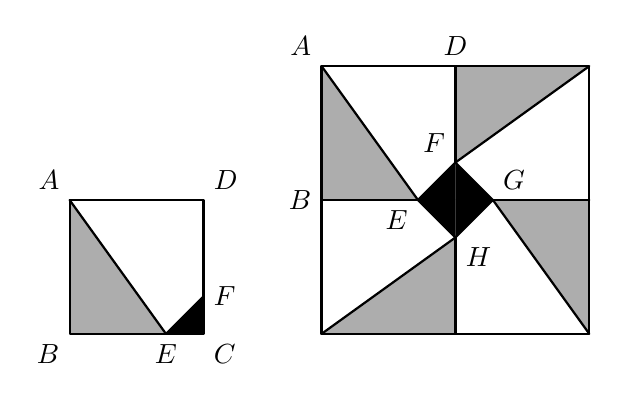
\begin{tikzpicture}[line cap=round,line join=round,thick]
\begin{scope}[scale=1.7]
  \fill[black!32] (0,1)--(0,0)--(.72,0)--cycle;
  \fill[black] (1,0)--(1,.28)--(.72,0)--cycle;
  \draw (0,0) rectangle (1,1); \draw (0,1)--(.72,0)--(1,.28);
  \node[above left] at (0,1) {$A$}; \node[below left] at (0,0) {$B$};
  \node[below right] at (1,0) {$C$}; \node[above right] at (1,1) {$D$};
  \node[below] at (.72,0) {$E$}; \node[right] at (1,.28) {$F$};
\end{scope}
\begin{scope}[xshift=3.2cm,scale=1.7]
  \foreach \angle in {0,90,180,270}{
    \begin{scope}[shift={(1,1)},rotate=\angle,shift={(-1,-1)}]
      \fill[black!32] (0,2)--(0,1)--(.72,1)--cycle;
      \fill[black] (1,1)--(1,1.28)--(.72,1)--cycle;
      \draw (0,2)--(.72,1)--(1,1.28);
    \end{scope}
  }
  \draw (0,0) rectangle (2,2);
  \draw (0,1)--(.72,1) (1.28,1)--(2,1) (1,0)--(1,.72) (1,1.28)--(1,2);
  \node[above left] at (0,2) {$A$}; \node[left] at (0,1) {$B$};
  \node[above] at (1,2) {$D$};
  \node[below left] at (.72,1) {$E$}; \node[above left] at (1,1.28) {$F$};
  \node[above right] at (1.28,1) {$G$}; \node[below right] at (1,.72) {$H$};
\end{scope}
\end{tikzpicture}
\end{center}
\nopagebreak[4]
\Needspace{0.4\textheight}
\end{question}
\begin{question}
\gkti{20}\textbf{（本题满分 $18$ 分）} 本题共有3个小题，第1小题满分6分，第2小题满分4分，第3小题满分8分。

通常用 $a$、$b$、$c$ 分别表示 $\triangle ABC$ 的三个内角 $A$、$B$、$C$ 所对边的边长，$R$ 表示 $\triangle ABC$ 的外接圆半径。

(1) 如图，在以 $O$ 为圆心、半径为2的 $\odot O$ 中，$BC$ 和 $BA$ 是 $\odot O$ 的弦，其中 $BC=2$，$\angle ABC=45^\circ$，求弦 $AB$ 的长；

(2) 在 $\triangle ABC$ 中，若 $\angle C$ 是钝角，求证：$a^2+b^2<4R^2$；

(3) 给定三个正实数 $a$、$b$、$R$，其中 $b\leq a$。问：$a$、$b$、$R$ 满足怎样的关系时，以 $a$、$b$ 为边长、$R$ 为外接圆半径的 $\triangle ABC$ 不存在、存在一个或存在两个（全等三角形算作同一个）？在 $\triangle ABC$ 存在的情况下，用 $a$、$b$、$R$ 表示 $c$。
\nopagebreak[4]
\begin{center}% Q20: source PDF p3; only BA and BC, AB is not a diameter.
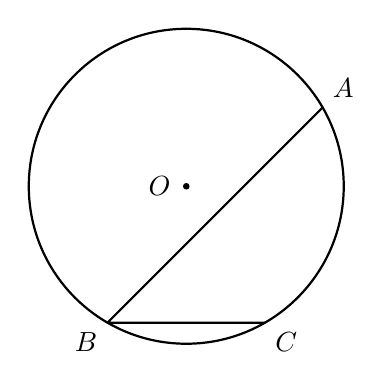
\begin{tikzpicture}[line cap=round,line join=round,thick]
\coordinate (O) at (0,0);
\coordinate (A) at (30:2); \coordinate (B) at (240:2); \coordinate (C) at (300:2);
\draw (O) circle[radius=2]; \draw (A)--(B)--(C);
\fill (O) circle[radius=1.2pt]; \node[left=2pt] at (O) {$O$};
\node[above right] at (A) {$A$}; \node[below left] at (B) {$B$};
\node[below right] at (C) {$C$};
\end{tikzpicture}
\end{center}
\nopagebreak[4]
\end{question}
\begin{question}
\gkti{21}\textbf{（本题满分 $18$ 分）} 本题共有3个小题，第1小题满分4分，第2小题满分6分，第3小题满分8分。

\Needspace{5\baselineskip}
我们在下面的表格内填写数值：先将第1行的所有空格填上1；再把一个首项为1、公比为 $q$ 的数列 $\{a_n\}$ 依次填入第一列的空格内；然后按照“任意一格的数是它上面一格的数与它左边一格的数之和”的规则填写其它空格。

\nopagebreak[4]
\[
\begin{array}{|c|c|c|c|c|c|}
\hline
 & \text{第1列} & \text{第2列} & \text{第3列} & \cdots & \text{第}n\text{列} \\ \hline
\text{第1行} & 1 & 1 & 1 & \cdots & 1 \\ \hline
\text{第2行} & q & & & & \\ \hline
\text{第3行} & q^2 & & & & \\ \hline
\cdots & \cdots & & & & \\ \hline
\text{第}n\text{行} & q^{n-1} & & & & \\ \hline
\end{array}
\]

(1) 设第2行的数依次为 $B_1,B_2,\cdots,B_n$，试用 $n$、$q$ 表示 $B_1+B_2+\cdots+B_n$ 的值；

(2) 设第3列的数依次为 $c_1,c_2,c_3,\cdots,c_n$，求证：对于任意非零实数 $q$，$c_1+c_3>2c_2$；

(3) 请在以下两个问题中选择一个进行研究（只能选择一个问题，如果都选，被认为选择了第一问）。

① 能否找到 $q$ 的值，使得(2)中的数列 $c_1,c_2,c_3,\cdots,c_n$ 的前 $m$ 项 $c_1,c_2,c_3,\cdots,c_m$（$m\geq3$）成为等比数列？若能找到，$m$ 的值有多少个？若不能找到，说明理由。

② 能否找到 $q$ 的值，使得填完表格后，除第1列外，还有不同的两列数的前三项各自依次成等比数列？并说明理由。

\end{question}